\documentclass[18pt]{beamer}
\usepackage[utf8]{inputenc}
\usepackage{templates/mytemplate}
\usepackage{templates/beamerthemekit}
\usepackage{graphicx}
\usepackage{microtype}
\usepackage{listings}
\usepackage{color}
\usepackage{hyperref}
\usepackage{multicol}
\usepackage{siunitx}
\usepackage{physics}
\usepackage{appendixnumberbeamer}
\usepackage{hyperref}

\hypersetup{
  linkcolor  = kit-blue100,
  urlcolor  = kit-blue100,
  colorlinks = true
 }

\title{Difference in Kinematic Distributions in GCR August  2017 MC Sample and Data}
\subtitle{Belle 2 Weekly Tracking Meeting}
\author{\underline{Michael Eliachevitch}}
\date{2017-11-17}
\titleimage{transparent}
\institute{ETP - KIT}

\begin{document}

  \selectlanguage{english}
  
  \begin{frame}
  \titlepage
\end{frame}

\begin{frame}
  \frametitle{What I did}
  \begin{itemize}
  \item at F2F tracking meeting I showed data from GCR Juli 2017 with back-to-back TSF trigger and used self-generated MC without trigger simulation
  \item recently MC samples with have trigger simulation became available for both GCR 2017 Juli and August runs 
  \item I received August MC with single TSF simulation and data and plan to use it for my cosmic based tracking study
  \item did my own reconstruction because I look at the \texttt{NonMergedRecoTracks},
  \item compared  distribution of kinematic variables from the non-merged track fits in MC and data
  \item unexpected differences, in particular in $z_0$ and $d_0$.
  \end{itemize}
\end{frame}

\begin{frame}
  \frametitle{My Track Parameter Distributions in MC and Data}
  \includegraphics[width=0.45\textwidth]{figures/gcr_august_2017_d0_distribution_normed=False.pdf}
  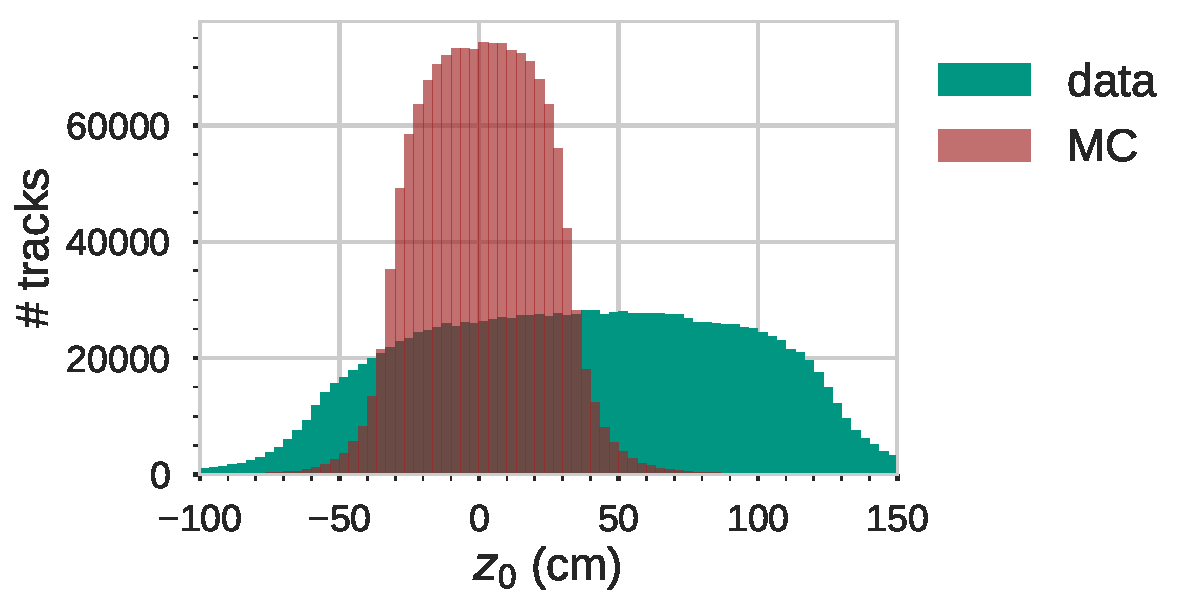
\includegraphics[width=0.45\textwidth]{figures/gcr_august_2017_z0_distribution_normed=False.pdf}\\
  \includegraphics[width=0.45\textwidth]{figures/gcr_august_2017_phi0_distribution_normed=False.pdf}
  \includegraphics[width=0.45\textwidth]{figures/gcr_august_2017_tan_lambda_distribution_normed=False.pdf}
\end{frame}

\begin{frame}
  \frametitle{Distributions from GCR Run Coordinator Report from B2GM}
  Taken from \href{https://kds.kek.jp/indico/event/25459/session/52/contribution/25/material/slides/0.pptx}{talk} by Shoji Uno at B2GM on 12 October 2017
  \centering
  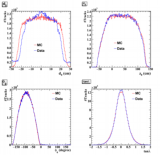
\includegraphics[width=0.6\textwidth]{figures/trackparam_distributions_from_b2gm_grc_run_coordinator_talk_2017-10-09.pdf}
\end{frame}

\begin{frame}
  \frametitle{Issues}
  \begin{itemize}
  \item My $z_0$ is much narrower on MC than on data. In the B2GM talk, the distribution looked narrower on data than what I reproduced, but wider in MC, all in all more similar.
  \item My $d_0$ MC distribution also looks different from data and from the B2GM talk
  \item Tail (?) in my $\tan \lambda$ distribution on data.
  \item My plots are from non-merged tracks, but I checked the distributions for the merged tracks, too, and they show the same issues.
  \end{itemize}
\end{frame}

\begin{frame}
  \frametitle{Questions}
  \begin{itemize}
  \item What exactly is shown in the plots from the B2GM? How are the track parameters extracted?
  \item Is the MC from the B2GM plots different from mine? Where is it located?
  \item What was the accept box in the MC creation?
  \item Are there somewhere else plots with more data?
  \item Write an E-Mail to Karim / the DP group?
  \end{itemize}
\end{frame}


\appendix
\backupbegin

\begin{frame}
  \begin{center}
    \huge Backup
  \end{center}
\end{frame}

\begin{frame}[allowframebreaks]
  \frametitle{Side by side comparison}
  \includegraphics[width=0.4\textwidth]{figures/gcr_august_2017_d0_distribution_normed=False.pdf}
  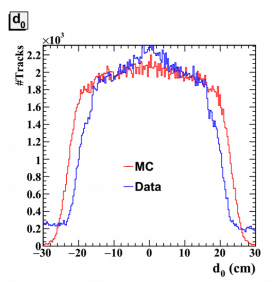
\includegraphics[width=0.35\textwidth]{figures/b2gm_d0.png}\\
  
  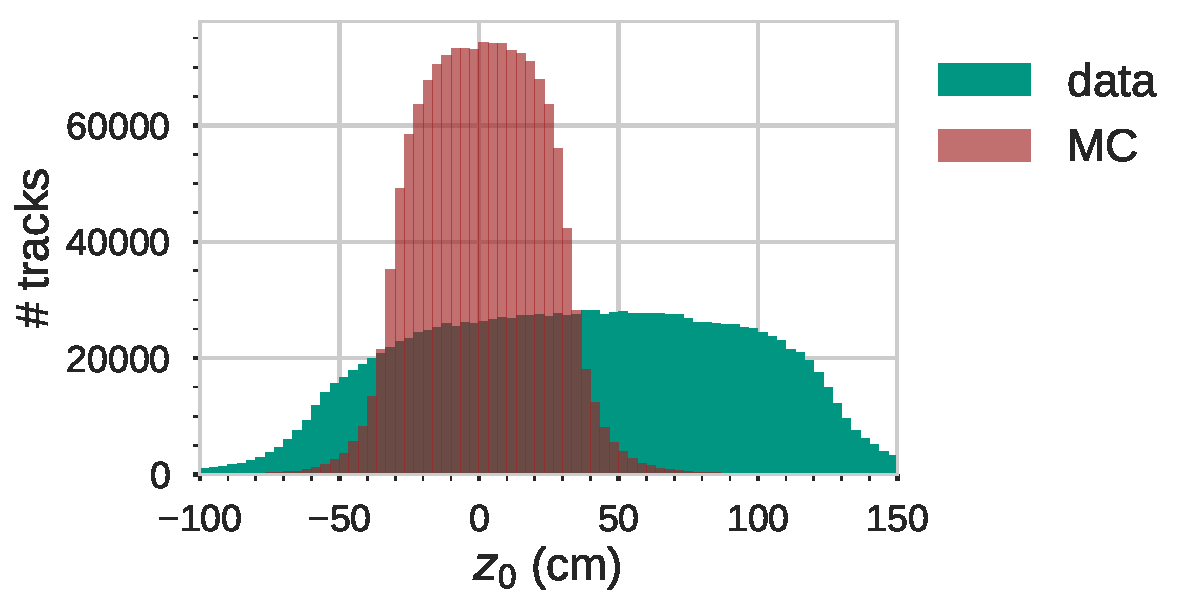
\includegraphics[width=0.4\textwidth]{figures/gcr_august_2017_z0_distribution_normed=False.pdf}
  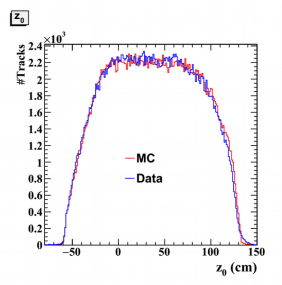
\includegraphics[width=0.35\textwidth]{figures/b2gm_z0.png}\\
  
  \includegraphics[width=0.4\textwidth]{figures/gcr_august_2017_phi0_distribution_normed=False.pdf}
  \includegraphics[width=0.35\textwidth]{figures/b2gm_phi0.png}\\
  
  \includegraphics[width=0.4\textwidth]{figures/gcr_august_2017_tan_lambda_distribution_normed=False.pdf}
  \includegraphics[width=0.35\textwidth]{figures/b2gm_tanlambda.png}\\
\end{frame}

\begin{frame}
  \frametitle{$p_T$ distribution}
  \includegraphics[width=0.7\textwidth]{figures/gcr_august_2017_pt_distribution_normed=False.pdf}
\end{frame}
      

\end{document}

%%% Local Variables:
%%% mode: latex
%%% TeX-master: t
%%% End:
